


\multiproblem{huh}{
  \begin{enumerate}
    %
	%
	\item A particle accelerates uniformly from rest, so that after 10 seconds it has achieved a speed of 15 ms$^{-1}$.
      \begin{enumerate}
        \item {Find the acceleration of the particle\A{ $a=\frac{v-u}{t}=\frac{15-0}{10}=1.5$ ms$^{-2}$} }
        \item{Find the distance covered\A{ $s=\frac{1}{2}(u+v)t=\frac{1}{2}(15)10=74$ m}}
      \end{enumerate}
    %
	%
	\item
	  The particle then decelerates uniformly to rest, covering another 45 m in the process.
      \begin{enumerate}
        \item Find the speed as a function of the distance covered for the whole journey (accelerating and decelerating)
          \A{\\ For the first part of the journey $v(s)^2=u^2+2as$,
		    so $v(s)=\sqrt{3S}$ for $0\leq s \leq 75$.\\
            For the second part of the journey $v_2^2=u_2^2+2a_2s_2$,
		    $a_2=\frac{v_2^2-u_2^2}{2s_2}=\frac{-15^2}{90}$, $s_2=45$ m.\\
            so $v(s)^2=u_2^2+2a_2 (s-75)$. Rearranging, $v(s)=\sqrt{600-2s}$ for $75<s\leq120$.
		    So
		    $$v(s)=
		      \begin{cases} 
                \sqrt{3s} & 0\leq s\leq 75 \\
                \sqrt{600-2s} & 75< s\leq 120
              \end{cases}.
            $$
		  }
        \item Plot this function
		  \A{\\
            \begin{center}
              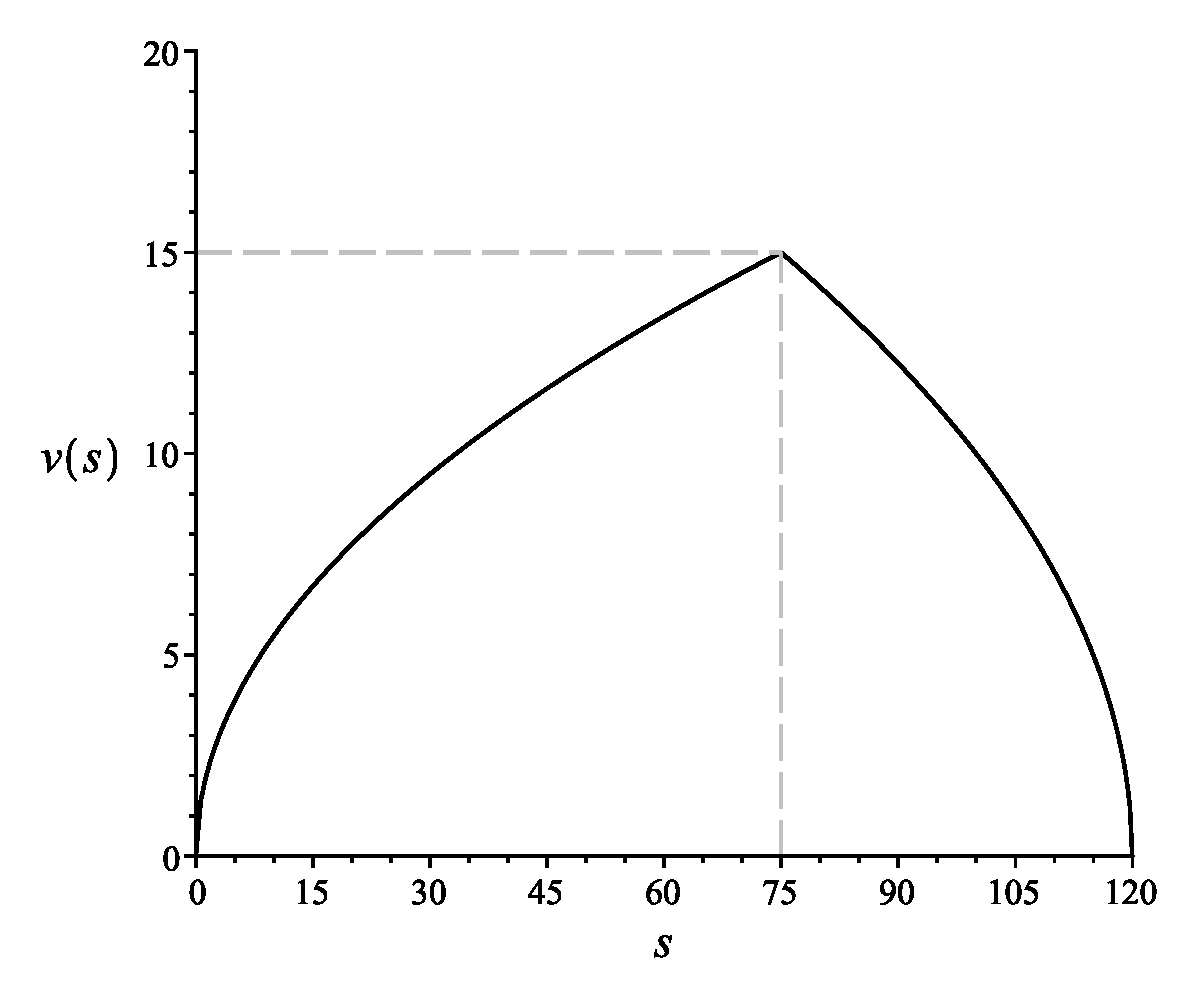
\includegraphics[scale=0.3]{v(s).eps}
            \end{center}
		  }
      \end{enumerate}
	%
    %	
  \end{enumerate}
}

\multiproblem{huh2}{ A projectile is fired off a a cliff of height 5 m at a speed of 5 ms$^{-1}$
\begin{figure}[htbp]
\centering
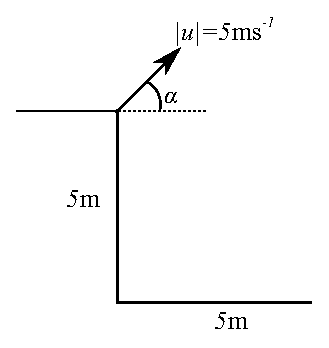
\includegraphics[]{cliff.eps}
\end{figure}
		\begin{enumerate}
    		\item{ 	At what angle from the horizontal $\alpha$ must the projectile be fired in order for it to land 5m from the base of the cliff?\A{\\
			$\underline{s}=(5,-5)^{T}$, $\underline{u}=(5\cos \alpha,5\sin \alpha)^{T}$ and $\underline{a}=(0,-g)^{T}$. If we use S(2) vertically and horizontally we can solve for $\alpha$\\
			Horizontally:\\
			$s_x=5=5 \cos \alpha t$, so $t=\sec \alpha$ \\
			Vertically:\\
			$s_y=-5=5\sin \alpha t -\frac{1}{2}g t^2$\\
			Substituting our result for $t$:
			$-5=5\sin \alpha \sec \alpha -\frac{1}{2}g \sec^2 \alpha$\\
			$-5=5 \tan \alpha -5 \sec^2 \alpha=5 \tan \alpha -5 (1+\tan^2 \alpha)$\\
			$0=\tan \alpha-\tan^2 \alpha$\\
			So either $\tan \alpha=0$ or $\tan \alpha =1$, meaning $\alpha=0$ or $\alpha=45^o=\pi/4$ radians respectively.}}
    \item{Sketch the trajectory/trajectories found in (a)\A{ \begin{figure}[htbp]
\centering
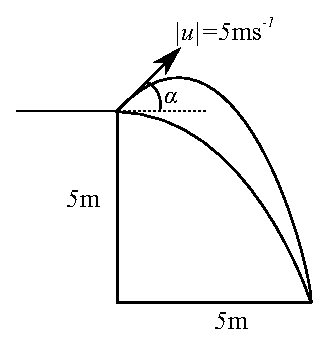
\includegraphics[]{cliff_traj.eps}
\end{figure}}}
    \item{ At what angle must the projectile be fired in order to be in the air for 1 second?\A{\\We can simply look at the projectile vertically, $s_y=-5=5\sin\alpha \times 1 -\frac{1}{2}g \times 1$. So
	$0=\sin \alpha$. Looking at the configuration, the correct solution is $\alpha=0$}}
\item{For general $\alpha$ find an expression for the distance of the projectile from its initial position as a function of time $t$\A{\\
$s_x=5t\cos \alpha$ and $s_y=5t\sin \alpha - 5t^2$. The distance can be found by $d=\sqrt{s_x^2+s_y^2}$\\
$d=\sqrt{25t^2 \cos^2 \alpha + 25t^2 \sin^2 \alpha - 50 t^3 \sin \alpha +25t^4}$\\
$d=5t\sqrt{1 - 2t \sin \alpha +t^2}$ for $t\geq0$}} 
  \end{enumerate}}


\multiproblem{huh3}{ 
A projectile is fired off a a cliff of height $h$, onto a hill, with an initial velocity of $$\underline{u}=(u,0)^{\mathrm{T}} \mathrm{ms}^{-1}$$
\begin{figure}[htbp]
\centering
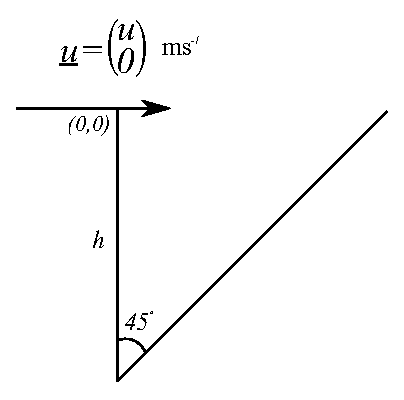
\includegraphics[]{cliff_hill.eps}
\end{figure}
		\begin{enumerate}
    		\item{ 	Show that the time in the air is $$T=\frac{-u+\sqrt{u^2+2gh}}{g}$$\A{The vertical displacement is given by $s_y=-\frac{1}{2}gt^2$ the horizontal $s_x=ut$\\
			We know that at the impact at $t=T$, $s_y=h-s_x$, so\\
			(1) $s_x=uT$\\
			(2) $s_x-h=-\frac{1}{2}gT^2$\\
			(1)-(2) $h=uT+\frac{1}{2}gT^2$\\
			Solving,we find $$T=\frac{-u\pm\sqrt{u^2 +2gh}}{g}$$\\
			We want the positive time solution so $$T=\frac{-u+\sqrt{u^2 +2gh}}{g}$$
			}}
    \item{Using the previous result, find the position vector at which the projectile hits the slope as a function of $h,u$ and $g$.\A{\\We found that $s_x=ut$ so at impact$$s_x=uT=\frac{-u^2+u\sqrt{u^2 +2gh}}{g}$$\\
	Furthermore, on the slope, we have that $$s_y=s_x-h=\frac{-u^2+u\sqrt{u^2 +2gh}}{g}-h$$So the position vector  is given by 
	$$\underline{p}_I=\left(\frac{-u^2+u\sqrt{u^2 +2gh}}{g},\frac{-u^2+u\sqrt{u^2 +2gh}}{g}-h\right)^T$$}}
    \item{ What are the limit of this position as $u\to \infty$ and $u\to 0$\A{\\
	This can either be found by intuition or mathematically finding the limits.\\
	Intuitively, as $u\to \infty$ the time taken to reach the slope tends to zero, and so the distance the projectile falls tends to zero (at a faster rate $s_y=\mathcal{O}(t^2)$). Therefore we can deduce that the position vector $\underline{p}\to (h,0)^T$.\\
	As $u\to 0$ the projectile can be considered as simply falling vertically, and so the distance the projectile travels horizontally tends to zero. We know that $s_y=s_x-h$, therefore we can deduce that the position vector $\underline{p}\to (0,-h)^T$.\\
	Mathematically, the limit as $u\to 0$ can also be found in a few ways. We can find that the limit as $T\to0$ is finite $\sqrt{2h/g}$ and so $s_x=uT\to0$. We can then trivially find $\underline(p)\to(-h,0)^T$.
	The limit as $u\to \infty$ is far harder. Let us start by rearranging $$s_x=\frac{-u^2+u\sqrt{u^2 +2gh}}{g}=\frac{u^2}{g}\left(-1+\sqrt{1+\frac{2gh}{u^2}}\right)$$
	Now we need the expansion $$(1+z)^a=1+az+\frac{a(a-1)}{2!}z^2+...$$
	In the case where $a=\frac{1}{2}$
	$$(1+z)^\frac{1}{2}=1+\frac{1}{2}z-\frac{1}{8}z^2+...$$
	So
	$$s_x=\frac{u^2}{g}\left(-1+\left(1+\frac{1}{2}\frac{2gh}{u^2}-\frac{1}{8}\left(\frac{2gh}{u^2}\right)^2+...\right)\right)$$
	$$s_x=h-\frac{gh^2}{4u^2}+\mathcal{O}(u^{-4})...$$
	Therefore, the limit as $u\to\infty$ of $s_x=h$.
}}
\item{Find an expression for the distance of the projectile from its initial position as a function of time $t$} 
  \end{enumerate}}



\multiproblem{huh4}{ I am throwing a ball up to a friend on top of a roof 20 m above me.
\begin{enumerate}
\item{What is the minimum initial velocity with which I can throw the ball, so that it reaches my friend?}
\item{I now need the ball to reach my friend within 1 second. What is the minimum initial velocity with which I can throw the ball now? \A{}}
\item{If my friend misses the first opportunity to catch the ball, how long is it before they get another chance?}
\item{How quickly would I have to throw the ball to reach my friend if they were at a height $h$ in order to reach them within 1 second?}
\item{If my friend misses the first catch, how long before they have another opportunity to catch it now?} 
\end{enumerate}}



\multiproblem{huh5}{  This question deals with deriving the SUVAT equations. In general the differential equations relating displacement, velocity and acceleration of a body are given by $\frac{ds(t)}{dt}=v(t)$, and $\frac{dv(t)}{dt}=a(t)$.

\begin{enumerate}
\item Using these, and the fact that we are modeling a situation where the acceleration is constant, derive an expression for $v(t)$ and one for $s(t)$ by integration. (Your solutions will look slightly different to S(1) and S(2), briefly explain this difference).

\item Using your answers from (a), derive S(5).

\item Using separation of variables, show that the area under a velocity-time plot (the graph of $v(t)$) is equal to the displacement. Is this result valid even for non-constant acceleration?

\item Constant acceleration implies constant gradient on a velocity-time plot, use this and a sketch to verify S(3).

\item From Newton's First Law, constant acceleration implies constant force acting on the body. Write down expressions for work done and kinetic energy, and hence derive S(4). (You will need to use the fact that work done is equal to the change in kinetic energy)
\end{enumerate}}

\multiproblem{huh6}{ 
\begin{enumerate}
\item In an experiment I drive a car, mass $m$, from stationary to a flag 20m away applying constant acceleration of 4\mpssq. Find the time $t^*$ it takes me to reach the flag.

\item I repeat the experiment, but this time I see a hazard in the distance at time $\tau<t^*$ and immediately apply constant deceleration. Find an expression for $F$, the force required to bring the car to a stop at the flag, as a function of $\tau$. Sketch the graph of $F(\tau)$.

\item In another experiment, I drop a coin down a well which has a depth of 75\metres. Assuming the speed of sound is 300\mps, find the time at which I hear the coin hit the bottom. 
\end{enumerate}}


\multiproblem{huh7}{  This question concerns a popular firework device which can fire fireworks out at any angle to the horizontal. We treat these fireworks as projectiles with initial speed $u$ under acceleration due to gravity $g$. We want to find an analytic expression for the boundary of the `safe area', where no firework can reach.
\begin{enumerate}
\item Write down $\mathbf{u}=(u_x,u_y)$, the firework's initial velocity as an expression in $\theta$, the angle at which the firework is fired from.
\item If $\big(s_x(t), s_y(t)\big)$ is a firework's position at time $t$, show that the graph of a firework's trajectory is
\begin{equation}
	\label{eq:s_y}
	s_y = s_x \tan\theta - \frac{s_x^2g}{2v^2}\big(1+\tan^2\theta\big).
\end{equation}

\textit{Hint: Begin by finding $s_x$ and $s_y$ and then relate them by explicitly eliminating $t$.}

\item Equation \ref{eq:s_y} is the family of all possible firework trajectories. You can think of it as $s_y$ as a function of $s_x$, parametrised by a choice of $\theta\in[0,\pi]$. In other words for a particular choice of $\theta$, the graph of $s_y(s_x)$ is that firework's trajectory. Now, we want to maximise this set over $\theta$. Find $\frac{\partial s_y}{\partial \theta}$ and hence find the maximal $s_y$ position for any given $s_x$ position.

\textit{Hint: Instead, use the substitution $z=\tan\theta$ and maximise $s_y(s_x)$ with respect to $z$. Bonus question: think why this substitution is allowed by considering the graph of $\tan(\theta)$.}

\item  Sketch the safe area boundary that you have found.

\end{enumerate}}
